%\documentclass{article}
%\documentclass[aip,jcp,amsmath,amssymb,reprint]{revtex4-1}

\documentclass[conference]{IEEEtran}
\IEEEoverridecommandlockouts
% The preceding line is only needed to identify funding in the first footnote. If that is unneeded, please comment it out.
\usepackage{cite}
\usepackage{amsmath,amssymb,amsfonts}
%\usepackage{algorithmic}
\usepackage{graphicx}
\usepackage{textcomp}
\usepackage{xcolor}
\def\BibTeX{{\rm B\kern-.05em{\sc i\kern-.025em b}\kern-.08em
		T\kern-.1667em\lower.7ex\hbox{E}\kern-.125emX}}

\usepackage[utf8]{inputenc}
%\usepackage[ruled,vlined]{algorithm2e}
\usepackage{algpseudocode}
\usepackage{algorithm}
\usepackage{amsmath}
\usepackage{amssymb}

\newcommand{\pluseq}{\mathrel{+}=}
\newcommand{\minuseq}{\mathrel{-}=}
\newcommand{\asteq}{\mathrel{*}=}
\renewcommand{\algorithmiccomment}[1]{\hfill$\triangleright$\textit{#1}}

\title{CS7642 Project 1 report}
\author{Qinghui Ge}
\date{January 2020}

\begin{document}
	
	\maketitle
	
	\begin{abstract}
		In this report, I demonstrate my efforts in reproducing some of the results regarding $TD(\lambda)$ algorithm in Sutton's paper: \textit{Learning to Predict by the Methods of Temporal Differences} (1988)\cite{sutton1988learning}. I will explain in detail about my implementation of two experiments presented in the original paper, and the discuss the similarity and discrepancy in my results and that of Sutton's paper.
	\end{abstract}
	
	\section{Problem}
	In Sutton's paper\cite{sutton1988learning}, he proposed a new learning procedure called $TD(\lambda)$ and apply it to a random walk problem. Sutton first derived $TD(1)$, which is equivalent to the Widrow-Hoff procedure in the supervised learning context, but is formulated to be implemented incrementally and is able to make prediction on each time-step of a sequence. He then generalized $TD(1)$ by introducing a parameter $\lambda$. The resulting algorithm $TD(\lambda)$ has different weight update than any supervised learning method, and Sutton showed that in the random walk problem, $TD(\lambda)$ has better performance than the Widrow-Hoff procedure.
	
	The $TD(\lambda)$ update procedure for the weight parameter $\omega$ is:
	\begin{align}
		\omega &\leftarrow \omega + \sum_{t=1}^{T} {\Delta \omega_t} \notag\\
		&= \omega + \alpha \sum_{t=1}^{T}(P_{t+1} - P_{t})\sum_{k=1}^{t} \lambda^{t-k}\nabla_\omega P_k
		\label{eq:tdlm}
	\end{align}
	$P_t$ is a prediction of final observation $z$ at time step $t$, and $P_{T} = z$ if the sequence terminate at step $T$. The prediction is a function of state vector $x$ that defined by the parameter $\omega$. For example, if $P_t$ is a linear function of $x_t$, then $P_t$ = $\omega^T x_t$ and $\nabla_\omega P_t = x_t$.
	
	$\alpha$ in Eq.\ref{eq:tdlm} is the learning rate. The $\lambda$ parameter takes value from [0,1]. It effectively scales gradient of $k$ steps in the past by a factor of $\lambda^k$. $\lambda=1$ is the Widrow-Hoff limit. The sum in Eq.\ref{eq:tdlm} can be evaluated incrementally (using the sum of previous time step):
	\begin{align*}
		e_t &= \sum_{k=1}^{t} \lambda^{t-k}\nabla_\omega P_k \\
		& = \nabla_\omega P_t + \lambda \sum_{k=1}^{t-1} \lambda^{t-1-k}\nabla_\omega P_k \\
		& = \nabla_\omega P_t + \lambda e_{t-1}
	\end{align*}
	Putting this in the context of random walk, we have 7 states: A-G (see figure 1). A random walk sequence starts at center state D, and can take a left or right in each step, until ends in terminate states A or G. A sequence has outcome reward $z=0$ if it ends at A, and $z=1$ if it ends at G. At each time step, we can predict the expected outcome based on the current state. For example, if at time step $t$ we are at the center state $D$, we would predict $P_t = P_D = 0.5$ since the sequence is equally likely to end in A and G. If at time $t'$ we are at $F$, then we would expect $P_{t'}=P_F$ to be some number between 0.5 and 1, since the sequence is now more likely to end in G. In fact, we can prove that the expected out come for states B-F is ($\frac{1}{6}$, $\frac{1}{3}$, $\frac{1}{2}$, $\frac{2}{3}$, $\frac{5}{6}$).
	
	In Sutton's paper, the state vector are chosen to be unit vectors, that is $x_B = [1,0,0,0,0]$, $x_C = [0,1,0,0,0]$ ... $x_F = [0,0,0,0,1]$. In this case, $P_t$ is $\mathrm{seq}[t]^{th}$ element of $\omega$. Any other set of orthonormal basis vectors can be used to represent the states, but the exact forms of $P_t$ and $\nabla_\omega P_t$ have to be changed accordingly, and the elements of $\omega$ vector can not be directly interpreted as the expectation value of $z$ (one has to take the general form $\omega^T x$).
	
	
	\section{Implementation}
	In this section, I discuss my implementation of $TD(\lambda)$ method to solve the random walk problem, as well as problems I encountered during the process.
	
	Same as in Sutton's paper, I prepare 100 training sets, each containing 10 sequences of random walk. The pseudo-code for generating sequence is presented in Algorithm~\ref{algo:seq}. Although the sequences can be generated on-the-fly during training process, I prepare all training sets in the beginning, and use the same 100 training sets through all experiments. This is consistent with Sutton's setting.
	
	
	\begin{algorithm}[h!]
		\caption{Prepare Training Sets}
		\begin{algorithmic}
			\Function{generate\_sequence}{start, n\_state} 
			\State seq = [start]
			\State s = n\_state
			\While{s != 0 and s != n\_state-1}
			\State $s \pluseq (rand()<0.5?\; 1: -1)$
			\State seq.append(s)
			\EndWhile
			\State return seq
			\EndFunction
			
			\Comment Generate 100 training sets, each has 10 sequences. Each sequence starts at state D(idx=3) and ends at A(idx=0) or G(idx=6)
			
			\For {i in 1,2,...100}
			\For {j in 1,2,...10}
			\State all\_training\_set[i][j] = GENERATE\_SEQUENCE(start=3, n\_state=7)
			\EndFor
			\EndFor
			
		\end{algorithmic}
		\label{algo:seq}
	\end{algorithm}
	
	I explored two slightly different implementations of Eq.\ref{eq:tdlm} (described in Algorithm.~\ref{algo:dw1} and ~\ref{algo:dw2}). In each time step, we compute $\Delta \omega_t = \alpha * (P_{t+1}-P_t) * e_t$, where $\alpha$ is the learning rate, $P_t = \omega^T x_t = \omega[\mathrm{seq}[t]]$. $e_t$ is updated by scaling the previous $e_{t-1}$ by the factor $\lambda$, and adding $\Delta e_t = \nabla_\omega P_t = x_t$.
	
	The two algorithms differ in whether the weights of the terminate states $A$ and $G$ are trainable. In Algorithm~\ref{algo:dw1}, the first and last elements of $\omega$ vector are initialized to $z$ value of corresponding terminate states (0 and 1) and never get updated in the time-iteration. In Algorithm~\ref{algo:dw2}, the two elements are trainable, they get updated in the last time step when the terminate state is reached. These two elements can be initialized to 0.5 as other elements, and will approach 0 and 1 respectively given the training converges. The two algorithms gives similar results and I decided to stick with Algorithm~\ref{algo:dw1}, because it is slightly simpler and more efficient (as final signal needs to propagate through 1 less state). As Sutton didn't consider the error of first and last elements, and his state vectors only have 5 elements, I think Algorithm~\ref{algo:dw1} is also what Sutton used.
	
	\begin{algorithm}[h!]
		\caption{compute $\Delta\omega$ given a sequence}
		\begin{algorithmic}
			\Function{update}{$\omega$, seq, $\alpha$, $\lambda$} 
			\Statex \Comment {first and last element of $\omega$ should be initialized to the true observation value z (0 and 1 in this case), they will not be updated during the iteration.}
			\State $n_s$ = len($\omega$) 
			\State initialize $e_t = [0]*n_s$ 
			\State initialize $\Delta\omega = [0]*n_s$ 
			\For {t = 0,1,2...len(seq)-2}
			\State     $\Delta e = [0]*n_s$ 
			\State     $\Delta e[\mathrm{seq}[t]] = 1$ 
			\State     $e_t = \Delta e + \lambda e_t$ 
			\State     $P_t = \omega[\mathrm{seq}[t]]$ 
			\State     $P_{t+1} = \omega[\mathrm{seq}[t+1]]$ 
			\State     $\Delta \omega_t = \alpha * (P_{t+1} - P_t) * e_t$ 
			\State     $\Delta \omega \pluseq \Delta \omega_t $
			\EndFor
			\EndFunction
		\end{algorithmic}
		\label{algo:dw1}
	\end{algorithm}
	
	\begin{algorithm}[h!]
		\caption{Alternative way of compute $\Delta\omega$ given a sequence}
		\begin{algorithmic}
			\Function{update}{$\omega$, seq, $\alpha$, $\lambda$} 
			\Statex \Comment {In this case, first and last element of $\omega$ can be initialized like other elements and will be updated in the iteration.}
			\State $n_s$ = len($\omega$) 
			\State initialize $e_t = [0]*n_s$ 
			\State initialize $\Delta\omega = [0]*n_s$ 
			\For {t = 0,1,2...len(seq)-1}
			\State $\Delta e = [0]*n_s$ 
			\State $\Delta e[\mathrm{seq}[t]] = 1$ 
			\State $e_t = \Delta e + \lambda e_t$ 
			\State $P_t = \omega[\mathrm{seq}[t]]$ 
			\If {t!=len(seq)-1}
			\State $P_{t+1} = \omega[\mathrm{seq}[t+1]]$ 
			\Else:
			\State $P_{t+1}$ = (seq[t]==0? 0: 1)
			\EndIf
			\State     $\Delta \omega_t = \alpha * (P_{t+1} - P_t) * e_t$ 
			\State     $\Delta \omega \pluseq \Delta \omega_t $
			\EndFor
			\EndFunction
		\end{algorithmic}
		\label{algo:dw2}
	\end{algorithm}
	
	Sutton's two experiments follows different updating procedure given each training set (10 sequences). Algorithm~\ref{algo:ex1} shows the pseudo-code for experiment 1. The $\omega$ values are updated after seeing the entire training set, during which $\Delta \omega$ is accumulated. Each training set is presented multiple times until $\omega$ converges. In my implementation, the convergence criterion is set to be ... Smaller thresholds are experimented and did not bring significant change in results. It is worth noting that as $\Delta \omega$ is accumulated for the entire training set, experiment 1 typically needs a smaller learning rate than experiment 2. Sutton states in his paper that a small enough learning rate can ensure the convergence (but will certainly requires more iteration). In my implementation, I choose $\alpha=0.1$ and scale it by the size of training set. All training is able to converge under this effective learning rate (0.01), without reaching maximum iteration = 10000.
	
	
	\begin{algorithm}[h!]
		\caption{Experiment 1 $\omega$ update on single training set}
		\begin{algorithmic}
			\Function{training\_1}{$\alpha$, $\lambda$, training\_set} 
			\State $\omega$ = [0, 0,5, 0.5, 0.5, 0.5, 0.5, 1]
			\For {n = 1,2,3...max\_iteration}
			\For {seq in training\_set}
			\State $\Delta \omega \pluseq \mathrm{UPDATE}(\omega, \mathrm{seq}, \alpha/\mathrm{traing\_set\_size}, \lambda)$
			\EndFor
			\State $\omega \pluseq \Delta \omega$
			\If {sum(abs($\Delta \omega$)) $<$ thresh}
			\State break
			\EndIf
			\EndFor
			
			\State return RMSE($\omega$[1:-1], $\omega_{true}$)
			\EndFunction
		\end{algorithmic}
		\label{algo:ex1}
	\end{algorithm}
	
	In experiment 2 (see Algorithm~\ref{algo:ex1}), each training set is only presented once, and $\omega$ vector is updated for each sequence of a training set.
	
	\begin{algorithm}[h!]
		\caption{Experiment 2 $\omega$ update on single training set}
		\begin{algorithmic}
			\Function{training\_2}{$\alpha$, $\lambda$, training\_set} 
			\State $\omega$ = [0, 0,5, 0.5, 0.5, 0.5, 0.5, 1]
			\For {seq in training\_set}
			\State $\omega \pluseq \mathrm{UPDATE}(\omega, \mathrm{seq}, \alpha, \lambda)$
			\EndFor
			
			\State return RMSE($\omega$[1:-1], $\omega_{true}$)
			\EndFunction
		\end{algorithmic}
		\label{algo:ex2}
	\end{algorithm}
	
	Both Algorithm~\ref{algo:ex1} and Algorithm~\ref{algo:ex2} return the root-mean-squared error (RMSE) between $\omega$ and the theoretical values ([$\frac{1}{6},\frac{1}{3},\frac{1}{2},\frac{2}{3},\frac{5}{6}$]) after training on a given training set. Finally, given a parameter set \{$\alpha$ and $\lambda$\}, both experiment 1 and 2 use Algorithm~\ref{algo:final} to compute the average and standard deviation of RMSE in 100 training set.
	
	\begin{algorithm}[h!]
		\caption{Compute the average and standard deviation of RMSE error in all training set}
		\begin{algorithmic}
			\Function{compute\_error}{$\alpha$, $\lambda$, all\_training\_set} 
			\State errors = []
			\For {training\_set in all\_training\_set}
			\State rmse = TRAINING\_1/2($\alpha$, $\lambda$, training\_set)
			\State errors.append(rmse)
			\EndFor
			
			\State return mean(errors), std(errors)
			\EndFunction
		\end{algorithmic}
		\label{algo:final}
	\end{algorithm}
	
	\section{Results}
	Before trying to reproduce Sutton's results, I did a quick sanity check on my UPDATE algorithm: I averaged the $\omega$ of 1000 training sets with size 100. The average $\omega$ vector is [0.162, 0.331, 0.495, 0.666, 0.835, 1], which is very close to theoretical value, with RMSE=0.00337.
	
	I reproduced figure 3,4,5 in Sutton's paper. In addition to average RMSE, I also plot the standard error (estimated by $SE=\frac{std(RMSE's)}{\sqrt{n\_training\_set}}=\frac{std(RMSE's)}{10}$) in order to have a sense of statistical significance. 
	
	Figure 3 plots the average RMSE vs different choices of $\lambda$. Both my and Sutton's figure show the optimal $\lambda$ is $\lambda=0$, and the error increases as $\lambda$ increases toward 1 (Widrow-Hoff limit). Despite agreeing on general trend, my RMSE ranges from around 0.11-0.18, while Sutton's ranges from 0.19-0.25. Initially I suspect this is due to randomness of training sets preparation, however, this is unlikely given the standard errors $SE<0.01$ (this is consistent with Sutton, who also reports $SE<0.01$). In addition, a few different run changing random seed do not alter my results significantly.
	
	\begin{figure}
		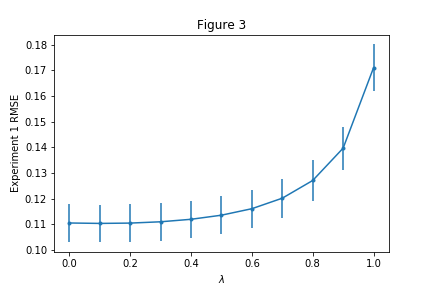
\includegraphics[height=2.5in]{figure3.png} 
		\caption{Replication of Figure 3 in Sutton's paper. Experiment 1 average RMSE over 100 training set for different $\lambda$ values. The error bar is $\pm 1\times SE$ computed from 100 training set.}
		\label{fig:3}
	\end{figure}
	
	Figure 4 shows the average RMSE while altering learning rate $\alpha$, at four different $\lambda$ values (0,0.3,0.8,1). When $\alpha=0$, there is no update on $\omega$, so the error for $\lambda's$ is the RMSE of the initial guess ([0.5,0.5,0.5,0.5,0.5]), which is 0.2357. The general shape of the lines are similar to Sutton's. Errors of $\lambda=1$ increase quickly as $\lambda$ increases. Errors of $\lambda = 0.3$ and $0.8$ are relatively insensitive to $\alpha$. The $\alpha$'s that give minimum error for the above 4 $\lambda$ values are (0.2, 0.2, 0.1, 0.05), while in Sutton's paper there were (0.3, 0.3, 0.15, 0.05). The standard error for the larger $\alpha$ values are quite large, so the lines in this region can change significantly between different runs. As I understand the last sequence in each training set would have stronger influence on $\omega$, especially when $\alpha$ is large, causing more variance between training sets.
	
	\begin{figure}
		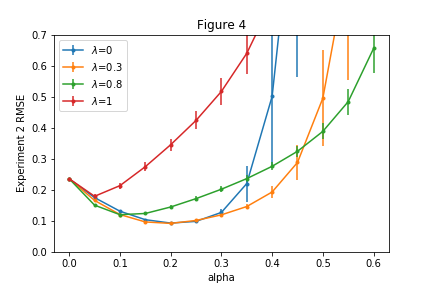
\includegraphics[height=2.5in]{figure4.png} 
		\caption{Replication of Figure 4 in Sutton's paper. Experiment 2 average RMSE over 100 training set, for different learning rate $\alpha$ given $\lambda = 0,0.3,0.8,1$.}
		\label{fig:3}
	\end{figure}
	
	Figure 5 shows the smallest error for each $\lambda$ with optimized learning rate $\alpha$. $\lambda=0.2$ has smallest error. In Sutton's paper, the minimum falls between 0.2-0.3. The minimal error is around 0.09, while Sutton's minimum is above 0.1. In both my and Sutton's results, $\lambda=1$ gives largest error, but maximum value is different. Overall, the results shares similar pattern as in Sutton's paper, with noticeable difference in the range of RMSE values. Again, the small standard error (especially for smaller $\lambda$'s) makes me think that the discrepancy is unlikely due to randomness in training sets.
	
	\begin{figure}
		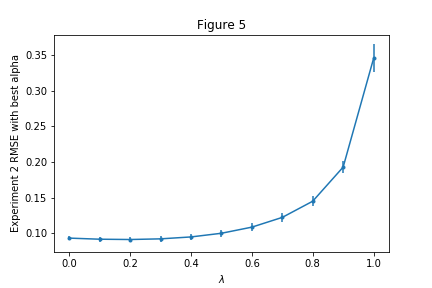
\includegraphics[height=2.5in]{figure5.png} 
		\caption{Replication of Figure 5 in Sutton's paper. Experiment 2 average RMSE over 100 training set, for different $\lambda$ values at optimal $\alpha$.}
		\label{fig:3}
	\end{figure}
	
\section{conclusion}

	
\bibliographystyle{IEEEtran}
\bibliography{reference}

\end{document}
